% NEVER CHANGE THIS TEMPLATE FORMATS
% PAPER MUST BE UNDER 7 PAGES INCLUDING REFERENCES
%
% IEEE AIoT 2026: Conference Paper Submission
% DOUBLE-BLIND SUBMISSION
% Template: IEEE Conference Template (June 2024 revision)
% Track:    Track 3: Edge, Cloud, and Fog Computing in IoT
%
% =====================================================================
% PAGE LIMIT: 6 pages content + references, total <= 7 pages.
% =====================================================================

\documentclass[conference]{IEEEtran}
\IEEEoverridecommandlockouts
% Template version as of 6/27/2024

\usepackage{cite}
\usepackage{amsmath,amssymb,amsfonts}
\usepackage{algorithmic}
\usepackage{graphicx}
\usepackage[caption=false,font=footnotesize]{subfig}
\usepackage{textcomp}
\usepackage{xcolor}
\usepackage{booktabs}
\usepackage{multirow}
\usepackage{array}
\usepackage{url}
\usepackage{flushend}
\usepackage{pgfplots}
\usepgfplotslibrary{groupplots}
\pgfplotsset{compat=1.17}

\def\BibTeX{{\rm B\kern-.05em{\sc i\kern-.025em b}\kern-.08em
    T\kern-.1667em\lower.7ex\hbox{E}\kern-.125emX}}

\begin{document}

\title{Negative-Frame Prevalence, Not Architecture, Governs
       False-Alarm Suppression in Edge AIoT Object Detection}

\author{\IEEEauthorblockN{Anonymous Authors}
\IEEEauthorblockA{Institution redacted for double-blind review}}

\maketitle

%------------------------------------------------------------------
\begin{abstract}
%------------------------------------------------------------------
Deep learning detectors deployed in continuous edge Artificial
Intelligence of Things (AIoT) sensing face extreme temporal class
imbalance: over 80\% of operational frames contain no targets.
Training with background-only (negative) frames suppresses false
alarms, but prior work tunes negative-frame ratios for one detector
architecture at a time, leaving open whether these settings transfer
across designs.
We present a cross-architecture study of four matched-capacity
($2.3$--$2.6$\,M parameter) nano-scale detectors from the You Only
Look Once (YOLO) family: YOLO11n (hybrid convolution-attention),
YOLO26n (structural reparameterization), YOLO12n (area attention),
and YOLOv10n (dual-label-assignment, non-maximum suppression (NMS)-free),
evaluated on a 15,723-frame driver-monitoring corpus with 80.9\%
natural negative prevalence.
Sweeping five negative-frame ratios (0\%--80\%), we find that
false-alarm suppression reaches up to $25.7\times$
across architectures, with all four converging
to a narrow operational band ($3.14$--$7.08$\,FP/1k, false positives
per 1,000 frames) at 80\% negatives, with no corresponding drop in
foreground recall (Spearman $\rho = +0.012$, not significant).
At a fixed 40\% ratio, hard-mined negatives reduce false alarms by
$52.6\%$--$67.8\%$ for attention-based and dual-assignment models,
and by $33.3\%$ for the pure-convolutional model.
These results indicate that negative-frame prevalence, not
architecture or inference latency, is the primary lever for
operational reliability in edge AIoT sensing.
\end{abstract}

\begin{IEEEkeywords}
edge AIoT, object detection, false-alarm suppression, negative-frame
training, YOLO, hard-negative mining, driver monitoring
\end{IEEEkeywords}

%==================================================================
\section{Introduction}
\label{sec:intro}
%==================================================================

Vision systems in continuous edge Artificial Intelligence of Things
(AIoT) sensing must process video
for hours at a time under severe foreground-background class
imbalance~\cite{lin2017focal}, yet the safety-critical events they
are built to detect are rare. In vehicular driver monitoring systems
(DMS), for example, cues such as phone use, drinking, or yawning
occupy only a small share of the video stream~\cite{sengupta2023dms},
while more than 80\% of frames show nothing of interest.

This imbalance changes what counts as good performance for an edge
detector. Mean average precision (mAP) on a curated, target-dense
benchmark says little about how the same detector behaves across
hours of routine footage; what matters operationally is whether the
detector stays silent when there is nothing to detect. A high
false-alarm rate drains battery and thermal budgets, wastes cellular
bandwidth, and causes driver alert fatigue~\cite{sengupta2023dms,chen2023falsealert}.

Training with background-only (negative) frames is a well-established
remedy for false alarms. Practitioner guidance suggests keeping
negative frames at around 0--10\% of the training set~\cite{ultralytics2024tips},
while studies in camera-trap ecology and open-world object detection
report that omitting negative frames severely degrades false-alarm
resilience~\cite{beery2018terra,oksuz2021imbalance}. This guidance,
however, comes from single-architecture studies: whether a
negative-frame ratio or a curation strategy that works well for one
detector transfers to another remains an open question. If
negative-frame sensitivity depends on architecture, then detector
choice and dataset curation cannot be treated as independent design
decisions.

We address this gap with a focused, cross-architecture study.
We fine-tune four matched-capacity ($2.3$--$2.6$\,M parameter)
nano-scale detectors from the YOLO family: YOLO11n~\cite{jocher2024yolo11},
YOLO26n~\cite{ultralytics2026yolo26}, YOLO12n~\cite{tian2025yolo12},
and YOLOv10n~\cite{wang2024yolov10}, spanning hybrid
convolution-attention, structural reparameterization, area-attention,
and dual-label-assignment (NMS-free) designs. On a 15,723-frame
in-cabin DMS corpus with 80.9\% natural negative prevalence, we ask:

\begin{itemize}
\item \textbf{RQ1 (Ratio Sensitivity):} How does the negative-frame
  ratio affect false-alarm suppression across architectures, and does
  the best-performing ratio differ by paradigm?
\item \textbf{RQ2 (Curation Quality):} At a fixed reference ratio
  ($r_{\mathrm{ref}} = 40\%$), does replacing random negatives with
  hard-mined negatives of equal count suppress false alarms further?
\end{itemize}

Our contributions are threefold. First, to our knowledge, this is
among the first cross-architecture negative-frame ratio sweeps on a
safety-critical AIoT dataset, spanning four detector paradigms.
Second, we run a controlled hard-negative mining benchmark at matched
cardinality ($r_{\mathrm{ref}} = 40\%$), isolating sample difficulty
from dataset size. Third, we pair an empirical latency benchmark with
an analytical translation from FP/1k to projected hourly nuisance
alerts ($\mathcal{A}_h$), showing that data curation---not inference
speed---determines whether a detector is usable in continuous
deployment.

%==================================================================
\section{Related Work}
\label{sec:related}
%==================================================================

\textbf{Foreground-Background Imbalance.}
Class imbalance in object detection is typically addressed by
loss reweighting~\cite{lin2017focal}, online hard-region
mining~\cite{shrivastava2016ohem,singh2018sniper}, dynamic sample
assignment~\cite{zhang2020atss}, and representation-drift
tracking~\cite{wang2019consistent}. These techniques target
candidate regions \textit{within} positive, object-containing
images. In continuous AIoT video streams, the dominant failure mode
is different: entire frames contain zero targets yet provoke
spurious detections that waste edge compute, trigger unnecessary
uplink transmissions, and fatigue operators~\cite{sengupta2023dms,chen2023falsealert}.
A unified treatment of this image-level imbalance problem,
including its effect on open-world false-alarm rates, is provided
by Oksuz et al.~\cite{oksuz2021imbalance}.

\textbf{Lightweight Edge Detectors.}
Edge AIoT deployments require compact architectures capable of
real-time inference under strict compute and thermal
budgets~\cite{wang2023microedge}. Modern nano-scale detectors
differ fundamentally in how they aggregate spatial features: hybrid
convolutional-attention models (YOLO11~\cite{jocher2024yolo11})
combine C3k2 blocks with neck-level partial self-attention (C2PSA);
structural reparameterization models (YOLO26~\cite{ultralytics2026yolo26})
use multi-branch RepConv during training and fuse to a single
efficient kernel at inference; area-attention models
(YOLO12~\cite{tian2025yolo12}) apply partitioned horizontal and
vertical attention (A2C2f) for near-linear complexity global context;
and dual-assignment models (YOLOv10~\cite{wang2024yolov10}) eliminate
NMS via consistent one-to-one prediction heads. Evaluating these four
paradigms at matched parameter count ($2.3$--$2.6$\,M) isolates the
effect of feature-aggregation design on background suppression.

\textbf{Negative-Frame Training in AIoT.}
Practitioner guidelines advise including 0--10\% background
images~\cite{ultralytics2024tips}. Camera-trap studies show that
omitting background images causes open-world failure
modes~\cite{beery2018terra}. In human-object interaction, negative
pair scaling to 1000:1 is essential to prevent spatial spuriousness~\cite{gupta2019nofrills}.
In vehicular DMS~\cite{sengupta2023dms,fridman2019cognitive},
standard datasets~\cite{statefarm2016,ortega2020dmd} emphasize
positive-cue diversity, while deployed systems encounter vast
stretches of unannotated routine driving. Critically, no prior work
examines whether an optimal negative-frame ratio or hard-negative
curation strategy transfers across distinct detector architectures.
This paper fills that gap.

%==================================================================
\section{Methodology}
\label{sec:methodology}
%==================================================================

\subsection{Problem Formulation}
\label{subsec:formulation}

In a continuous edge AIoT video stream
$\mathcal{S} = \{X_t\}_{t=1}^T$, frames are partitioned into
positive frames ($\mathcal{D}_{\mathrm{pos}}$, containing annotated
driver-safety cues) and negative frames
($\mathcal{D}_{\mathrm{neg}}$, containing no targets). For a
detector $f_\theta$, bounding boxes predicted on frame $X$ and
filtered at operational confidence threshold $\tau \in (0,1]$ yield
the detection set $\hat{\mathcal{Y}}_\tau(X)$. Because negative
frames carry no ground truth ($Y = \emptyset$), any element of
$\hat{\mathcal{Y}}_\tau(X)$ is an operational false alarm.

We quantify deployment reliability via two metrics evaluated on the
held-out negative test set $\mathcal{D}_{\mathrm{test}}^{\mathrm{neg}}$
($1{,}272$ frames):
\begin{equation}
\mathrm{FP/1k} = \frac{1000}{|\mathcal{D}_{\mathrm{test}}^{\mathrm{neg}}|}
  \sum_{X \in \mathcal{D}_{\mathrm{test}}^{\mathrm{neg}}}
  |\hat{\mathcal{Y}}_\tau(X)|,
\label{eq:fp1k}
\end{equation}
and the projected hourly nuisance alert rate $\mathcal{A}_h$ at
camera frame rate $f_{\mathrm{FPS}}$ (frames per second):
\begin{equation}
\mathcal{A}_h = 3.6\, f_{\mathrm{FPS}}\, p_{\mathrm{neg}}\,
  \mathrm{FP/1k},
\label{eq:nuisance}
\end{equation}
where $p_{\mathrm{neg}} \approx 0.809$ is the operational negative
prevalence of our vehicular corpus. All false-alarm metrics are
evaluated at $\tau = 0.25$ and NMS intersection-over-union (IoU)
threshold of $0.70$. Standard accuracy metrics
($\mathrm{mAP}_{50}$, $\mathrm{mAP}_{50:95}$, precision P, recall
R) are reported at the maximum-$F_1$ operating point.

\subsection{Dataset and Partitioning}
\label{subsec:dataset}

Experiments use a 15,723-frame in-cabin DMS corpus captured under
diverse lighting conditions, vehicle interiors, driver subjects, and
camera viewpoints, with institutional consent and de-identification.
The dataset contains 3,001 positive frames annotated with verified
2D bounding boxes across four driver-cue classes:
\texttt{phone\_use} (2,437 frames, 81.2\%),
\texttt{drinking} (264 frames, 8.8\%),
\texttt{yawning} (159 frames, 5.3\%), and
\texttt{hand\_over\_mouth} (141 frames, 4.7\%).
The remaining 12,722 frames are background-only, yielding an 80.9\%
natural negative prevalence.

A stratified 80/10/10 split (seed\,=\,42) partitions the corpus
into: (1) a held-out test set of 1,572 frames (300 positive,
1,272 negative); (2) a held-out validation set of 1,572 frames
(300 positive, 1,272 negative); and (3) a training universe of
2,401 positive and 10,178 candidate negative frames. Both
evaluation sets preserve the natural 80.9\% negative dominance
and are fixed across all experiments.

\subsection{Detector Architectures}
\label{subsec:architectures}

Table~\ref{tab:architectures} summarizes the four nano-scale
detectors benchmarked in this study. All models operate within
$2.3$--$2.6$\,M parameters, $6.2$--$7.6$\,GFLOPs (giga
floating-point operations), and $22$\,ms latency on an NVIDIA
RTX 4060 Laptop graphics processing unit (GPU), ensuring that
result differences reflect architectural design rather than
parameter or compute budget.

\begin{table}[t]
\caption{Evaluated Detector Architectures (640\,$\times$\,640 Input)}
\label{tab:architectures}
\centering
\setlength{\tabcolsep}{1.6pt}
\begin{tabular}{lcccccc}
\toprule
\textbf{Model} & \textbf{Params} & \textbf{FLOPs} &
\textbf{Lat.$^*$} & \textbf{FPS$^*$} &
\textbf{Paradigm} & \textbf{Mechanism} \\
\midrule
YOLO11n  & 2.6\,M & 6.5\,G & 16.8\,ms & 59.6  & Hybrid    & C3k2 + C2PSA \\
YOLO26n  & 2.6\,M & 6.2\,G & 21.7\,ms & 46.1  & Rep.Conv  & RepConv \\
YOLO12n  & 2.6\,M & 7.6\,G & 21.3\,ms & 47.0  & Attn      & A2C2f (Area) \\
YOLOv10n & 2.3\,M & 6.6\,G & 7.7\,ms  & 129.2 & NMS-Free  & Dual-Label Head \\
\bottomrule
\end{tabular}
\vspace{1pt}
{\footnotesize $^*$Measured on NVIDIA RTX 4060 Laptop GPU (PyTorch,
batch\,=\,1, 640\,$\times$\,640, averaged over 200 iterations after
50 warm-up iterations).}
\end{table}

\subsection{Experimental Configurations}
\label{subsec:configurations}

\subsubsection{Axis 1 (RQ1) --- Negative-Frame Ratio Sweep}
Holding the positive core fixed at $|\mathcal{D}_{\mathrm{pos}}|
= 2{,}401$ frames, we construct five nested training subsets at
20-percentage-point increments: 0\% ($2{,}401$ total; 0 negative),
20\% ($3{,}001$; 600 negative), 40\% ($4{,}001$; 1,600 negative),
60\% ($6{,}003$; 3,602 negative), and 80\% ($12{,}005$; 9,604
negative). Subsets are strictly nested by increasing the negative
pool with seed\,=\,42, so later splits are supersets of earlier
ones. Axis~1 comprises 20 training runs (4 models $\times$ 5 ratios).

\subsubsection{Axis 2 (RQ2) --- Hard-Negative Curation}
For each architecture, a positive-only baseline ($r{=}0\%$) runs
inference over all 10,178 training negatives at $\tau{=}0.25$.
False-alarm frames are ranked by maximum predicted confidence
$s_{\max}(X)$, and the top $N_{\mathrm{target}}{=}1{,}600$ frames
form the curated hard-negative set (backfilled deterministically
from remaining negatives when needed). We evaluate curation at the
reference ratio $r_{\mathrm{ref}}{=}40\%$ with strictly matched
cardinality: $|\mathcal{D}_{\mathrm{train,hard}}^{(40\%)}|
= |\mathcal{D}_{\mathrm{train,rand}}^{(40\%)}| = 4{,}001$
frames, isolating sample difficulty from dataset volume. Axis~2
adds 8 training runs for a primary benchmark total of 28 runs.

\subsection{Training Protocol}
\label{subsec:protocol}

All models are fine-tuned from COCO (Common Objects in Context)-pretrained
checkpoints at $640 \times 640$ resolution, single precision (FP32),
using the AdamW optimizer ($\mathrm{lr}_0 = 0.00125$, weight
decay\,=\,0.0005, batch size\,=\,16) for 100 epochs with mosaic
augmentation disabled for the final 10 epochs
(\texttt{close\_mosaic=10}). Table~\ref{tab:training} summarizes
the frozen hyperparameters, which are held identical across all
models and ratio conditions.

\textit{Training-step note:} Fixing epoch count over variable
dataset sizes (2,401--12,005 frames) means the 80\% condition
receives approximately $5\times$ more gradient steps than the 0\%
condition. This confound is acknowledged; the convergence results
at 80\% should be interpreted as an upper bound on what extended
training with high negative prevalence can achieve rather than a
pure architectural effect.

\begin{table}[t]
\caption{Frozen Training Hyperparameters (All Models and Splits)}
\label{tab:training}
\centering
\setlength{\tabcolsep}{5pt}
\begin{tabular}{lc}
\toprule
\textbf{Hyperparameter} & \textbf{Value} \\
\midrule
Input resolution          & 640\,$\times$\,640 (FP32) \\
Batch / effective batch   & 16 / 16 \\
Training duration         & 100 epochs \\
Optimizer                 & AdamW ($\mathrm{lr}_0{=}0.00125$) \\
Weight decay              & 0.0005 \\
Mosaic cooldown           & Final 10 epochs \\
Random seed               & 42 (dual-seed: 42, 43 for $r \le 40\%$) \\
\bottomrule
\end{tabular}
\vspace{1pt}
{\footnotesize Hyperparameters are identical across all architectures
and ratio splits to isolate feature-aggregation design.}
\end{table}

%==================================================================
\section{Experimental Results}
\label{sec:results}
%==================================================================

\subsection{Ratio Sensitivity (RQ1)}
\label{subsec:rq1_results}

Table~\ref{tab:rq1} reports detection accuracy and operational
false-alarm rates across all ratio-sweep conditions on the held-out
test set (1,572 frames, 80.9\% negative prevalence).

\begin{table}[t]
\caption{Negative-Frame Ratio Sweep across Architectures (RQ1)}
\label{tab:rq1}
\centering
\setlength{\tabcolsep}{1.2pt}
\begin{tabular}{llccccc}
\toprule
\textbf{Det.} & \textbf{$r$} &
\textbf{$\mathrm{mAP}_{50}$} &
\textbf{$\mathrm{mAP}_{50\text{-}95}$} &
\textbf{P} & \textbf{R} &
\textbf{FP/1k} \\
\midrule
\multirow{5}{*}{YOLO11n}
& 0\%  & 0.9824 & 0.7570 & 0.8576 & 0.9787 & 67.22 \\
& 20\% & 0.9838 & 0.7524 & 0.9283 & 0.9814 & 31.05 \\
& 40\% & 0.9919 & 0.7711 & 0.9308 & 0.9831 & 22.01 \\
& 60\% & 0.9899 & \textbf{0.7723} & 0.9468 & 0.9806 & 9.83 \\
& 80\% & \textbf{0.9933} & 0.7606 & \textbf{0.9644} & 0.9766 & \textbf{4.72} \\
\midrule
\multirow{5}{*}{YOLO26n}
& 0\%  & 0.9170 & 0.7086 & 0.8557 & 0.9105 & 80.59 \\
& 20\% & 0.9729 & 0.7546 & 0.9306 & 0.9763 & 16.90 \\
& 40\% & 0.9726 & 0.7388 & 0.9224 & 0.9519 & 9.43 \\
& 60\% & 0.9660 & 0.7594 & \textbf{0.9587} & 0.9086 & 10.22 \\
& 80\% & \textbf{0.9736} & \textbf{0.7671} & 0.9217 & \textbf{0.9794} & \textbf{3.14} \\
\midrule
\multirow{5}{*}{YOLO12n}
& 0\%  & 0.9910 & 0.7496 & 0.9228 & 0.9823 & 45.20 \\
& 20\% & 0.9757 & 0.7449 & 0.8954 & 0.9863 & 35.77 \\
& 40\% & 0.9866 & 0.7659 & 0.9199 & 0.9949 & 18.86 \\
& 60\% & 0.9888 & \textbf{0.7766} & 0.9348 & \textbf{0.9960} & 9.43 \\
& 80\% & \textbf{0.9925} & 0.7529 & \textbf{0.9621} & 0.9767 & \textbf{7.08} \\
\midrule
\multirow{5}{*}{YOLOv10n}
& 0\%  & 0.9423 & 0.7287 & 0.9065 & 0.8831 & 57.39 \\
& 20\% & 0.9423 & 0.7270 & 0.8833 & 0.9400 & 21.23 \\
& 40\% & 0.9642 & \textbf{0.7568} & 0.8813 & \textbf{0.9788} & 14.94 \\
& 60\% & \textbf{0.9749} & 0.7525 & \textbf{0.9221} & 0.9758 & \textbf{4.72} \\
& 80\% & 0.9524 & 0.7384 & 0.9010 & 0.9024 & \textbf{4.72} \\
\midrule
\multicolumn{7}{l}{{\footnotesize\textit{Pooled correlation with neg.\ ratio ($N{=}20$)}}} \\
\midrule
\multicolumn{2}{l}{Spearman $\rho$} &
  \multicolumn{2}{c}{---} &
  \textbf{+0.546}$^{*}$ & +0.012$^{\text{n.s.}}$ &
  \textbf{$-$0.937}$^{***}$ \\
\multicolumn{2}{l}{Pearson $r$}   &
  \multicolumn{2}{c}{---} &
  \textbf{+0.628}$^{*}$ & +0.147$^{\text{n.s.}}$ &
  \textbf{$-$0.857}$^{***}$ \\
\bottomrule
\end{tabular}
\vspace{1pt}
{\footnotesize Dual-seed means (seed\,=\,42,43) for $r \!\le\! 40\%$;
single seed otherwise. FP/1k at $\tau{=}0.25$, IoU\,=\,0.70.
P/R at max-$F_1$; 1,272 neg.\ test frames.
Corr.\ block ($N{=}20$): pooled across models;
$^{*}p{<}0.05$, $^{***}p{<}10^{-4}$, n.s.: $p{>}0.50$.
Bold: best per architecture.}
\end{table}

\noindent\textbf{High-ratio convergence.}
At $r{=}0\%$, all models produce substantial false-alarm leakage
because background frames generate no positive anchor assignments
and thus no backpropagation gradients to suppress non-target
activations. As negative prevalence scales to $r{=}80\%$, all four
architectures converge to a narrow operational band
($3.14$--$7.08$\,FP/1k). This convergence is driven by a strong
monotonic inverse relationship between negative ratio and FP/1k
(pooled Spearman $\rho{=}-0.937$, $p{<}10^{-4}$; Pearson
$r{=}-0.857$, $p{<}10^{-4}$). Precision improves significantly
with ratio (Spearman $\rho{=}+0.546$, $p{<}0.05$), while foreground
recall remains statistically uncorrelated ($\rho{=}+0.012$,
$p{>}0.50$), confirming that background regularization suppresses
hallucinations without eroding target sensitivity.

\noindent\textbf{Architectural divergence at intermediate ratios.}
The path to convergence differs sharply by paradigm
(Fig.~\ref{fig:empirical_summary}a). YOLO26n (RepConv) drops from
80.59 to 9.43\,FP/1k by $r{=}40\%$ because localized, fused
convolutional filters rapidly learn to suppress prominent cabin
textures (steering-wheel rims, seatbelt buckles). In contrast,
YOLO11n, YOLO12n, and YOLOv10n require $r{=}60\%$--$80\%$ to
reach comparable suppression. Attention layers compute dense
pairwise or area-based feature correlations; without sufficient
background variety, they bind ambient cues such as windshield
reflections and headrest contours into spurious foreground
hypotheses. YOLOv10n's dual-assignment architecture must
simultaneously suppress over-assignment in both its auxiliary
one-to-many head and its one-to-one inference head, requiring
sustained negative supervision. Relative to the zero-negative
baseline, suppression factors reach $25.7\times$ for YOLO26n
($80.59 \to 3.14$\,FP/1k), $14.2\times$ for YOLO11n ($67.22 \to 4.72$),
$12.2\times$ for YOLOv10n ($57.39 \to 4.72$), and $6.4\times$ for
YOLO12n ($45.20 \to 7.08$).

\noindent\textbf{Foreground localization is preserved.}
$\mathrm{mAP}_{50:95}$ remains within the range $0.738$--$0.777$
across all ratio levels (Fig.~\ref{fig:empirical_summary}b). Because
negative frames carry no ground truth, bounding-box regression and
distribution focal loss~\cite{li2020gfl} receive no update from them; only the
classification branch tightens its decision boundary on background
cells.

\begin{figure*}[t]
\centering
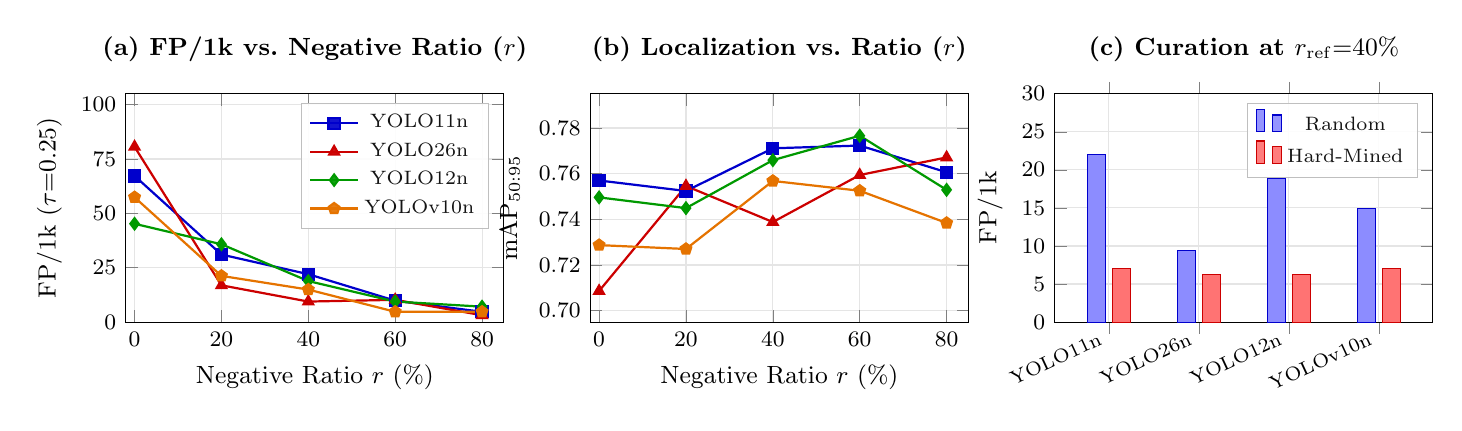
\begin{tikzpicture}
\begin{groupplot}[
  group style={group size=3 by 1, horizontal sep=1.1cm},
  scale only axis,
  width=4.8cm, height=2.9cm,
  tick label style={font=\footnotesize},
  label style={font=\small},
  title style={font=\small\bfseries, yshift=2pt},
  grid=major, grid style={gray!20}
]
% (a) FP/1k vs Ratio
\nextgroupplot[
  title={(a) FP/1k vs.\ Negative Ratio ($r$)},
  xlabel={Negative Ratio $r$ (\%)},
  ylabel={FP/1k ($\tau{=}0.25$)},
  xmin=-2, xmax=85, ymin=0, ymax=105,
  xtick={0,20,40,60,80},
  ytick={0,25,50,75,100},
  legend style={at={(0.96,0.96)}, anchor=north east,
    font=\scriptsize, fill=white, fill opacity=0.92, draw=gray!50}
]
\addplot[color=blue!80!black,   mark=square*,   thick]
  coordinates {(0,67.22)(20,31.05)(40,22.01)(60,9.83)(80,4.72)};
  \addlegendentry{YOLO11n}
\addplot[color=red!80!black,    mark=triangle*,  thick]
  coordinates {(0,80.59)(20,16.90)(40,9.43)(60,10.22)(80,3.14)};
  \addlegendentry{YOLO26n}
\addplot[color=green!60!black,  mark=diamond*,   thick]
  coordinates {(0,45.20)(20,35.77)(40,18.86)(60,9.43)(80,7.08)};
  \addlegendentry{YOLO12n}
\addplot[color=orange!90!black, mark=pentagon*,  thick]
  coordinates {(0,57.39)(20,21.23)(40,14.94)(60,4.72)(80,4.72)};
  \addlegendentry{YOLOv10n}

% (b) mAP50:95 vs Ratio
\nextgroupplot[
  title={(b) Localization vs.\ Ratio ($r$)},
  xlabel={Negative Ratio $r$ (\%)},
  ylabel={$\mathrm{mAP}_{50:95}$},
  xmin=-2, xmax=85, ymin=0.695, ymax=0.795,
  xtick={0,20,40,60,80},
  ytick={0.70,0.72,0.74,0.76,0.78},
  yticklabel style={/pgf/number format/fixed,
    /pgf/number format/precision=2,
    /pgf/number format/zerofill}
]
\addplot[color=blue!80!black,   mark=square*,   thick]
  coordinates {(0,0.7570)(20,0.7524)(40,0.7711)(60,0.7723)(80,0.7606)};
\addplot[color=red!80!black,    mark=triangle*,  thick]
  coordinates {(0,0.7086)(20,0.7546)(40,0.7388)(60,0.7594)(80,0.7671)};
\addplot[color=green!60!black,  mark=diamond*,   thick]
  coordinates {(0,0.7496)(20,0.7449)(40,0.7659)(60,0.7766)(80,0.7529)};
\addplot[color=orange!90!black, mark=pentagon*,  thick]
  coordinates {(0,0.7287)(20,0.7270)(40,0.7568)(60,0.7525)(80,0.7384)};

% (c) Random vs Hard-Mined Bar Chart
\nextgroupplot[
  title={(c) Curation at $r_{\mathrm{ref}}{=}40\%$},
  ybar=2.5pt, bar width=6.5pt,
  enlarge x limits=0.20,
  ylabel={FP/1k},
  symbolic x coords={YOLO11n,YOLO26n,YOLO12n,YOLOv10n},
  xtick=data,
  x tick label style={rotate=25, anchor=east, font=\scriptsize},
  ymin=0, ymax=30,
  ytick={0,5,10,15,20,25,30},
  legend style={at={(0.96,0.96)}, anchor=north east,
    font=\scriptsize, fill=white, fill opacity=0.92, draw=gray!50}
]
\addplot[fill=blue!45, draw=blue!80!black]
  coordinates {(YOLO11n,22.01)(YOLO26n,9.43)(YOLO12n,18.86)(YOLOv10n,14.94)};
  \addlegendentry{Random}
\addplot[fill=red!55,  draw=red!80!black]
  coordinates {(YOLO11n,7.08)(YOLO26n,6.29)(YOLO12n,6.29)(YOLOv10n,7.08)};
  \addlegendentry{Hard-Mined}
\end{groupplot}
\end{tikzpicture}
\caption{Cross-architecture results.
(a) FP/1k decreases monotonically as negative ratio $r$ increases,
converging to $3.14$--$7.08$\,FP/1k at $r{=}80\%$ across all
architectures; suppression trajectories at intermediate ratios are
paradigm-dependent.
(b) $\mathrm{mAP}_{50:95}$ is robust across all ratio levels
(${\ge}0.709$), confirming that background training does not erode
foreground localization.
(c) At matched cardinality ($r_{\mathrm{ref}}{=}40\%$, $N{=}4{,}001$),
hard-negative curation cuts FP/1k by 33\%--68\% depending on
architecture; attention and dual-assignment models gain most.
Line and marker coding in (a) and (b) is shared.}
\label{fig:empirical_summary}
\end{figure*}

\subsection{Hard-Negative Curation vs.\ Random Sampling (RQ2)}
\label{subsec:rq2_results}

Table~\ref{tab:rq2} compares hard-negative mining against uniform
random sampling at $r_{\mathrm{ref}}{=}40\%$ with matched
cardinality ($N{=}4{,}001$ frames). Values are dual-seed means
(seed\,=\,42, 43).

\begin{table}[t]
\caption{Hard-Negative Mining vs.\ Random at Matched Cardinality
  ($r_{\mathrm{ref}}{=}40\%$, RQ2)}
\label{tab:rq2}
\centering
\setlength{\tabcolsep}{4pt}
\begin{tabular}{llcccc}
\toprule
\textbf{Detector} & \textbf{Curation} &
\textbf{$\mathrm{mAP}_{50}$} &
\textbf{$\mathrm{mAP}_{50:95}$} &
\textbf{FP/1k} &
\textbf{$\%\,\Delta$} \\
\midrule
\multirow{2}{*}{YOLO11n}
& Random     & 0.9919 & 0.7711 & 22.01 & \multirow{2}{*}{\textbf{$-$67.8\%}} \\
& Hard-Mined & \textbf{0.9932} & \textbf{0.7738} & \textbf{7.08} & \\
\midrule
\multirow{2}{*}{YOLO26n}
& Random     & 0.9726 & 0.7388 & 9.43  & \multirow{2}{*}{\textbf{$-$33.3\%}} \\
& Hard-Mined & \textbf{0.9759} & \textbf{0.7518} & \textbf{6.29} & \\
\midrule
\multirow{2}{*}{YOLO12n}
& Random     & 0.9866 & 0.7659 & 18.86 & \multirow{2}{*}{\textbf{$-$66.7\%}} \\
& Hard-Mined & \textbf{0.9928} & \textbf{0.7839} & \textbf{6.29} & \\
\midrule
\multirow{2}{*}{YOLOv10n}
& Random     & 0.9642 & 0.7568 & 14.94 & \multirow{2}{*}{\textbf{$-$52.6\%}} \\
& Hard-Mined & \textbf{0.9788} & \textbf{0.7673} & \textbf{7.08} & \\
\bottomrule
\end{tabular}
\vspace{1pt}
{\footnotesize Evaluated on 1,272 negative test frames
($\tau{=}0.25$, matched $N{=}4{,}001$ training frames).
$\%\,\Delta$: relative change in FP/1k (hard-mined vs.\ random).
Bold marks best condition per architecture.}
\end{table}

\noindent\textbf{All architectures benefit from curation, but to different degrees.}
Hard-negative mining reduces FP/1k for every architecture; the
magnitude of the gain is strongly architecture-dependent
(Fig.~\ref{fig:empirical_summary}c).

\noindent\textit{Attention and dual-assignment models (YOLO11n, YOLO12n,
YOLOv10n):} These models achieve $52.6\%$--$67.8\%$ false-alarm
reductions alongside localization gains
($\mathrm{mAP}_{50:95}$ increasing by up to $+0.018$). Uniform
random sampling predominantly selects low-entropy background patches
(plain headrests, uniform window glass) that deliver negligible
gradient feedback to global query-key attention weights. Hard
negatives---featuring complex cabin reflections and partial driver
silhouettes---provoke spurious cross-attention activations, and
explicit training on them forces attention layers to decorrelate
these ambient patterns from true driver cues. For YOLOv10n, mined
negatives penalize over-assignment in the auxiliary one-to-many head,
sharpening the inference-time one-to-one branch.

\noindent\textit{Structural reparameterization (YOLO26n):}
Hard-negative mining still yields a meaningful $33.3\%$ reduction
($9.43 \to 6.29$\,FP/1k), but the absolute gain is smaller than
for attention models. YOLO26n's localized $3{\times}3$ RepConv
kernels rapidly learn dominant cabin textures from even random
negatives and saturate earlier; high-entropy hard negatives provide
useful but less incremental gradient signal because the model's
limited global receptive field cannot exploit long-range contextual
distinctions.

\noindent\textbf{Practical curation rule.}
The data indicate a clear architectural gradient in curation
sensitivity: attention and dual-assignment architectures derive large
gains from hard-negative mining at matched dataset size, while
structural reparameterization models benefit more modestly. In
resource-constrained settings where mining pipelines add engineering
overhead, random sampling is adequate for RepConv-based models;
for attention-based or dual-head models, the $52\%$--$68\%$
false-alarm reduction justifies the curation cost.

\subsection{Operational Deployment Cost}
\label{subsec:cost_results}

Table~\ref{tab:deployment} translates FP/1k values into projected
hourly nuisance alert rates $\mathcal{A}_h$ via~\eqref{eq:nuisance}
at three standard streaming frame rates.

\begin{table}[t]
\caption{Projected Nuisance Alerts per Hour ($\mathcal{A}_h$)}
\label{tab:deployment}
\centering
\setlength{\tabcolsep}{5pt}
\begin{tabular}{llccc}
\toprule
\textbf{Detector} & \textbf{Training Split} &
\textbf{5\,FPS} & \textbf{15\,FPS} & \textbf{30\,FPS} \\
\midrule
\multirow{2}{*}{YOLO11n}
& 0\% neg.\ baseline  & 979   & 2{,}938 & 5{,}875 \\
& 80\% neg.\ ratio    & 69    & 206     & 412     \\
\midrule
\multirow{2}{*}{YOLO26n}
& 0\% neg.\ baseline  & 1{,}174 & 3{,}521 & 7{,}042 \\
& 80\% neg.\ ratio    & \textbf{46} & \textbf{137} & \textbf{274} \\
\midrule
\multirow{2}{*}{YOLO12n}
& 0\% neg.\ baseline  & 658   & 1{,}975 & 3{,}949 \\
& 80\% neg.\ ratio    & 103   & 309     & 619     \\
\midrule
\multirow{2}{*}{YOLOv10n}
& 0\% neg.\ baseline  & 836   & 2{,}507 & 5{,}014 \\
& 80\% neg.\ ratio    & 69    & 206     & 412     \\
\bottomrule
\end{tabular}
\vspace{1pt}
{\footnotesize Modeled via~\eqref{eq:nuisance} using
$p_{\mathrm{neg}}{=}0.809$ and measured FP/1k from Table~\ref{tab:rq1}. Bold: lowest alert rate per frame-rate column.}
\end{table}

Without negative training, detectors trigger up to 7{,}042 nuisance
alerts per hour at 30\,FPS. Scaling negative frames to 80\% cuts
alert rates by up to 96.1\% without changing a single model
parameter. This analysis formalizes a key principle for edge AIoT
systems: \textbf{inference latency is architecture-bound; operational
reliability is curation-bound.} YOLOv10n achieves the fastest
inference ($7.7$\,ms, 129\,FPS), but without negative training its
alert rate ($5{,}014$/hr at 30\,FPS) makes it impractical for
continuous deployment. Data curation is the decisive design lever.

%==================================================================
\section{Discussion}
\label{sec:discussion}
%==================================================================

\subsection{Practical Guidelines}

The empirical results support two concrete recommendations for edge
AIoT practitioners deploying DMS or similar continuous-sensing
systems.

\noindent\textbf{1) Prioritize negative-frame prevalence.}
Regardless of architecture, the single most impactful decision is
ensuring that training data reflects operational negative prevalence.
Training at $r{=}80\%$ negatives reduces FP/1k by $7.3\times$--$25.7\times$
relative to the zero-negative baseline and converges all four
architectures to a narrow operational band ($3.14$--$7.08$\,FP/1k).
For teams with sufficient data and compute, $r{=}80\%$ is the clear
recommendation. For teams with constrained training budgets, $r{=}40\%$
already captures the bulk of this suppression (FP/1k
$\le 22$\,for all models) while using less than one-third the
negative volume of the 80\% split.

\noindent\textbf{2) Match curation strategy to detector family.}
At a fixed training budget ($r{=}40\%$, $N{=}4{,}001$ frames),
hard-negative mining reduces false alarms by $52.6\%$--$67.8\%$
for attention and dual-assignment models (YOLO11n, YOLO12n,
YOLOv10n) and by $33.3\%$ for the structural reparameterization
model (YOLO26n). All four architectures benefit from curation, but
the gain is proportional to the model's capacity for global feature
correlation. Teams deploying RepConv-based models can rely on simple
random background sampling without a mining pipeline; teams
deploying attention-based or dual-head models should invest in
hard-negative curation to realize the larger available gains.

\subsection{Limitations}

\begin{itemize}\setlength{\itemsep}{0pt}
\item \textbf{Training-step confound.}
  Fixing epoch count over dataset sizes of 2,401--12,005 frames
  means the 80\% condition receives approximately $5\times$ more
  gradient steps. Step-controlled ablations remain future work.
\item \textbf{Mining purity variation.}
  Hard-mined candidate pools contained 34.2\%--59.2\% verified
  false-alarm frames (remainder: backfilled random negatives).
  The practical ceiling for curation gain therefore exceeds our
  reported figures.
\item \textbf{Temporal correlation.}
  Consecutive frames share the same cabin interior and lighting.
  Near-ceiling $\mathrm{mAP}_{50} > 0.97$ may partly reflect
  within-vehicle rather than cross-vehicle generalization.
\item \textbf{Foreground class imbalance.}
  The positive core is dominated by \texttt{phone\_use} (81.2\%),
  so aggregate mAP primarily tracks majority-class performance.
\item \textbf{Single-platform latency.}
  Latency is profiled on an NVIDIA RTX 4060 Laptop GPU. Target
  embedded platforms such as the NVIDIA Jetson Orin Nano will show
  different absolute values and relative rankings.
\end{itemize}

%==================================================================
\section{Conclusion}
\label{sec:conclusion}
%==================================================================

This paper investigated the joint effect of negative-frame
prevalence and hard-negative curation on false-alarm suppression
across four matched-capacity ($2.3$--$2.6$\,M parameter) YOLO
detectors in a continuous edge AIoT driver-monitoring task.

Three findings have immediate practical relevance. First, high
negative prevalence ($r{=}80\%$) is the single most effective lever
for suppressing false alarms: it reduces FP/1k by up to $25.7\times$
and drives all four architectures to a narrow operational band
($3.14$--$7.08$\,FP/1k) without eroding foreground recall (Spearman
$\rho{=}+0.012$, not significant). Second, suppression trajectories
at intermediate ratios diverge substantially by paradigm: structural
reparameterization models converge fast and early, while attention and
dual-assignment models require higher negative densities. This means
that detector selection and dataset curation are coupled design
decisions, not independent ones. Third, hard-negative mining at matched
cardinality yields large additional gains for attention and dual-assignment
models ($52.6\%$--$67.8\%$) but a more modest gain for the RepConv
model ($33.3\%$), providing a concrete heuristic for when to invest in
mining pipelines.

Together, these results shift the design-time question from
``which architecture has the best mAP?'' to ``which
architecture--curation combination achieves an acceptable hourly
nuisance alert rate at my deployment frame rate?'' Future work should
control for gradient steps across ratio conditions, evaluate
step-controlled schedules, extend the analysis to outdoor IoT sensing
domains, and explore confidence-calibration methods that can close
the remaining gap at the $r{=}40\%$ operating point.

%==================================================================
\section*{Acknowledgment}
%==================================================================
Acknowledgment omitted for double-blind review.

%==================================================================
% Bibliography
%==================================================================
\bibliographystyle{IEEEtran}
\bibliography{references}

\end{document}
